\documentclass[11pt,a4paper]{article}
\usepackage[utf8]{inputenc}
\usepackage[margin=1in]{geometry}
\usepackage{amsmath,amssymb,amsfonts}
\usepackage{graphicx}
\usepackage{tikz}
\usetikzlibrary{shapes,arrows,positioning,fit,calc,decorations.pathreplacing}
\usepackage{pgfplots}
\pgfplotsset{compat=1.18}
\usepackage{hyperref}
\usepackage{booktabs}
\usepackage{array}
\usepackage{float}

\title{PAI: A Novel Debt-Native Blockchain Protocol}
\author{PAI Protocol}
\date{\today}

\begin{document}

\maketitle

\begin{abstract}
PAI is a debt-native blockchain protocol that introduces a novel lending primitive built around non-transferable-in-default debt instruments. The protocol enables deposits of external assets to create debt-tracked instruments, generates loanable currencies derived from those deposits, and enforces strict debt obligations through immutable records. A custom consensus mechanism called \textit{Custom Attested Bundle} coordinates block production through sealed-bid auctions between paired producers and a rotating reputation-weighted committee. The system employs block-relevant validation against a shared replicated ledger, enforces one-transaction full debt settlement on instrument transfers with automatic burning on failure, and implements liquidation through pools with arbitrage mechanisms. The native currency PAI has a dynamic supply with fee burning and rewards distributed to network participants. The protocol further introduces a bounty lifecycle: when a depositor withdraws before unpaid loans are settled, a bounty is created from the withdrawn value and auctioned on-chain, with settlement to the highest bidder or, absent bids, proportional distribution and timed burning. This paper presents the complete system design, economic mechanisms, and security considerations.
\end{abstract}

\tableofcontents
\newpage

\section{Introduction}
Traditional blockchain systems lack native primitives for debt creation, enforcement, and liquidation in a unified manner. PAI addresses this gap by treating debt as a first-class primitive embedded at the protocol level. Rather than relying solely on smart contracts for lending logic, PAI encodes debt obligations, value mechanics, and liquidation paths directly into the protocol state machine.

The protocol introduces several innovations: (1) deposit-derived debt instruments with immutable history, (2) a custom consensus model combining pairwise production with committee attestation, (3) block-relevant validation that maintains security while limiting computational scope, (4) strict transfer mechanics requiring full debt settlement in a single transaction, (5) automatic liquidation escalation through pools to arbitrageurs, and (6) a ratio-based value factor mechanism, and (7) a bounty lifecycle that auctions withdrawn value when loans remain unpaid.

\section{System Overview}
PAI operates as a distributed system where network participants maintain identical copies of a shared replicated immutable ledger. All state transitions are append-only and fully auditable through immutable history records. The protocol enforces economic invariants at the consensus and execution layers, ensuring that debt obligations cannot be circumvented and that failed settlements trigger predetermined consequences.

\begin{figure}[H]
\centering
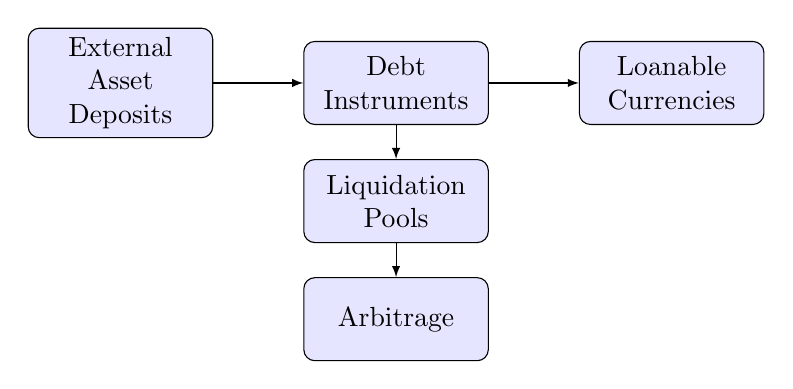
\begin{tikzpicture}[node distance=1.5cm, auto,
    block/.style={rectangle, draw, fill=blue!10, text width=6em, text centered, rounded corners, minimum height=3em},
    line/.style={draw, -latex}]
\node [block] (deposits) {External Asset Deposits};
\node [block, right of=deposits, xshift=2cm] (debt) {Debt Instruments};
\node [block, right of=debt, xshift=2cm] (loans) {Loanable Currencies};
\node [block, below of=debt] (liquidation) {Liquidation Pools};
\node [block, below of=liquidation] (arb) {Arbitrage};
\path [line] (deposits) -- (debt);
\path [line] (debt) -- (loans);
\path [line] (debt) -- (liquidation);
\path [line] (liquidation) -- (arb);
\end{tikzpicture}
\caption{Core economic flow in PAI}
\label{fig:coreflow}
\end{figure}

\section{Network Architecture}
\subsection{Node Roles}
PAI distinguishes between two primary node roles:

\begin{itemize}
\item \textbf{Block Producers}: Collect transactions, assemble blocks, maintain the shared replicated ledger, and verify attestations from validators.
\item \textbf{Validators}: Verify transaction validity against block-relevant state, produce attestations, and maintain identical copies of the shared replicated ledger.
\end{itemize}

Both roles maintain complete copies of the shared replicated immutable ledger. However, validation is performed only on transactions relevant to the current block, enabling efficient operation without requiring full-chain reprocessing.

\subsection{Shared Replicated Ledger}
The shared replicated ledger serves as the canonical source of truth maintained identically across all network participants. Properties include:
\begin{itemize}
\item Append-only immutability
\item Complete transaction and state history
\item Block-relevant indexing for efficient validation
\item Cryptographic commitments over state
\end{itemize}

\subsection{Block-Relevant Validation}
Rather than validating all historical state, nodes construct per-block state views containing only touched accounts, assets, and instruments. This approach maintains security guarantees while reducing validation scope to the minimal set required for correctness.

\section{Consensus: Custom Attested Bundle}
PAI employs \textit{Custom Attested Bundle} consensus, a hybrid model combining auction-based selection, pairwise production, and committee attestation.

\subsection{Sealed-Bid Auction}
For each block, eligible participants submit sealed bids to secure production rights. The auction proceeds in two phases:

\begin{enumerate}
\item \textbf{Commit Phase}: Participants submit commitments $C_i = H(b_i \| \eta_i)$ where $b_i$ is the bid amount in PAI and $\eta_i$ is a random nonce.
\item \textbf{Reveal Phase}: Participants reveal $(b_i, \eta_i)$, allowing verification against commitments.
\end{enumerate}

\subsection{Pair Selection}
From revealed bids, the highest bidder is selected as the block producer, and a second distinct participant is selected as the paired validator. A participant cannot be paired with themselves. The winning bid amount is paid if selected.

\subsection{Committee Formation}
A rotating committee of fixed size $k=4$ is selected from remaining eligible participants using reputation-weighted selection. The committee excludes members of the active pair, preventing collusion between producers and validators.

\subsection{Attestation and Quorum}
The paired validator produces an attestation of block validity after performing block-relevant validation against the shared replicated ledger. The block producer verifies this attestation against the same ledger state. Finalization requires quorum from the pair and majority support from the committee.

\begin{figure}[H]
\centering
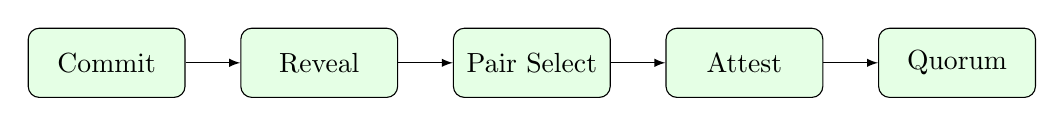
\begin{tikzpicture}[node distance=1.2cm, auto,
    phase/.style={rectangle, draw, fill=green!10, text width=5em, text centered, rounded corners, minimum height=2.5em},
    line/.style={draw, -latex}]
\node [phase] (commit) {Commit};
\node [phase, right of=commit, xshift=1.5cm] (reveal) {Reveal};
\node [phase, right of=reveal, xshift=1.5cm] (select) {Pair Select};
\node [phase, right of=select, xshift=1.5cm] (attest) {Attest};
\node [phase, right of=attest, xshift=1.5cm] (quorum) {Quorum};
\path [line] (commit) -- (reveal);
\path [line] (reveal) -- (select);
\path [line] (select) -- (attest);
\path [line] (attest) -- (quorum);
\end{tikzpicture}
\caption{Custom Attested Bundle consensus flow}
\label{fig:consensus}
\end{figure}

\section{Asset Deposits \& Debt Instruments}
\subsection{Deposit Mechanism}
Users deposit any external bridged asset into the protocol. Upon deposit confirmation, the protocol creates a debt-tracked instrument linked to the deposit. The deposit amount is split according to consensus parameters into three components:
\begin{itemize}
\item Loanable portion for currency creation
\item Reserve/backup portion
\item Interest pool portion
\end{itemize}

\subsection{Debt Instruments}
Each deposit generates a unique debt instrument with the following properties:
\begin{itemize}
\item Immutable history of all events (deposits, loans, repayments, transfers, liquidations)
\item Collateral backing from the original deposit
\item Associated loanable currency
\item Tracked debt balance and interest obligations
\item Value factor determining economic weight
\item Status indicating active, liquidating, burned, or paid-off state
\end{itemize}

The instrument history is append-only and cannot be modified, ensuring complete auditability of all debt-related events.

\section{Lending \& Interest}
Loanable currencies are created from deposits and can be issued against debt instruments. Interest accrues according to the rate established at instrument creation. Repayments must be made in the original currency context, with interest calculated as:

\begin{equation}
I = P \cdot \frac{r_{bps}}{10000}
\end{equation}

where $P$ is principal and $r_{bps}$ is the interest rate in basis points. Repayment updates the debt balance, adds events to the immutable history, and contributes to value factor restoration.

\section{Liquidation \& Arbitrage}
\subsection{Liquidation Triggers}
When debt obligations become unserviceable according to protocol rules, automatic liquidation is triggered. The debt instrument transitions to liquidating status and the debt escalates through the liquidation system.

\subsection{Liquidation Pools}
Liquidation pools are structured with a single provider instrument for aggregate accounting and fungible pool shares for depositors. Key mechanics:
\begin{itemize}
\item Depositors receive proportional shares representing claims on pool assets
\item Interest from lending activities distributes proportionally to shareholders
\item Pools provide liquidity for debt repayment during liquidation
\item All pool accounting is optimized for block-relevant validation
\end{itemize}

\subsection{Arbitrage Mechanism}
When pool liquidity is insufficient or for efficiency, debt is assigned to arbitrageurs as temporary instruments. Arbitrage rules are strictly enforced:

\begin{itemize}
\item \textbf{Profit retention}: If the arbitrageur repays the full debt from arbitrage proceeds, they retain remaining profits
\item \textbf{Loss absorption}: If the arbitrageur fails to recoup the full debt amount, they assume full liability for that debt
\item \textbf{Asset liquidation}: Failed arbitrageurs must liquidate remaining arbitrage assets to repay the debt
\item \textbf{Liability limitation}: Arbitrageurs only assume liability upon failure to recoup, never for debts not initially assigned
\end{itemize}

The escalation path follows: automatic liquidation $\rightarrow$ liquidation pool $\rightarrow$ arbitrageur assignment.

\begin{figure}[H]
\centering
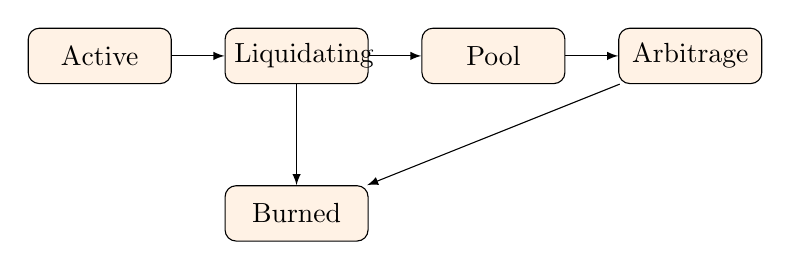
\begin{tikzpicture}[node distance=1cm, auto,
    state/.style={rectangle, draw, fill=orange!10, text width=4.5em, text centered, rounded corners, minimum height=2em},
    line/.style={draw, -latex}]
\node [state] (active) {Active};
\node [state, right of=active, xshift=1.5cm] (liq) {Liquidating};
\node [state, right of=liq, xshift=1.5cm] (pool) {Pool};
\node [state, right of=pool, xshift=1.5cm] (arb) {Arbitrage};
\node [state, below of=liq, yshift=-1cm] (burn) {Burned};
\path [line] (active) -- (liq);
\path [line] (liq) -- (pool);
\path [line] (pool) -- (arb);
\path [line] (liq) -- (burn);
\path [line] (arb) -- (burn);
\end{tikzpicture}
\caption{Liquidation escalation and burn paths}
\label{fig:liquidation}
\end{figure}

\section{Debt Instruments \& Trading}
\subsection{Transfer Restrictions}
Debt instruments are non-transferable in the standard sense and cannot be treated as conventional digital collectibles. Trading is permitted only under strict conditions enforced at the protocol level.

\subsection{One-Transaction Settlement Requirement}
When transferring a debt instrument, the receiver must pay all outstanding debts plus accrued interest in a single transaction. This requirement is enforced atomically:
\begin{enumerate}
\item Transfer request is evaluated
\item If outstanding debt exists ($D_{total} > 0$), receiver must provide full payment in same transaction
\item If full payment not provided, dealing currencies noted on the instrument are permanently burned
\item Instrument is marked burned and becomes permanently unusable
\item If full payment provided, debts are satisfied and transfer proceeds
\end{enumerate}

\subsection{Burning Mechanism}
Burning is permanent and irreversible. When triggered:
\begin{itemize}
\item All dealing currencies noted on the instrument are destroyed
\item The instrument status becomes burned
\item The instrument cannot be used for any economic activity
\item Burn events are recorded in immutable history
\item Burned currencies are not recoverable or redistributed
\end{itemize}

\subsection{Profit Distribution on Sale}
If a loan has been paid in full with interest, special profit distribution rules apply upon instrument sale:
\begin{itemize}
\item The seller receives the paid-off loaned currency amounts plus interest
\item The other mint holder receives a more valuable instrument due to improved value factor
\item These effects are reflected in the value factor mechanics
\end{itemize}

\section{Value Factor Mechanics}
\subsection{Definition}
The value factor $V$ represents the economic value of a debt instrument relative to its obligations, determined by the ratio between available collateral backing and total minted currencies:

\begin{equation}
V_t = \frac{C_{avail}(t)}{M_{total}(t)} \cdot \rho(t)
\end{equation}

where $C_{avail}$ is available collateral backing, $M_{total}$ is total currencies minted from the instrument, and $\rho(t)$ represents repayment restoration effects.

\subsection{Behavior}
\begin{itemize}
\item \textbf{Minting effect}: As more currencies are minted from an instrument, $M_{total}$ increases relative to $C_{avail}$, causing $V$ to decrease
\item \textbf{Repayment restoration}: When currencies are repaid, $C_{avail}$ increases and the repayment credit $\rho$ restores value
\item \textbf{Full repayment}: Paying off loans in full with interest affects value distribution on subsequent sales
\item \textbf{Tracking}: Value factor is tracked on-chain and all changes are recorded in immutable history
\end{itemize}

The value factor is bounded such that $0 \leq V \leq 1$ under normal conditions, with restoration mechanisms preventing permanent value collapse through repayment.

\begin{figure}[H]
\centering
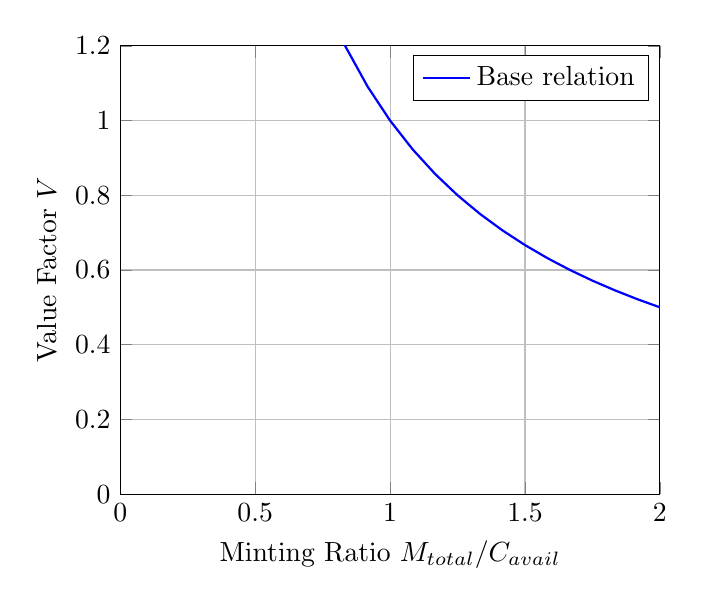
\begin{tikzpicture}
\begin{axis}[xlabel={Minting Ratio $M_{total}/C_{avail}$}, ylabel={Value Factor $V$}, xmin=0, xmax=2, ymin=0, ymax=1.2, grid=major]
\addplot[blue, thick, domain=0:2]{1/x};
\addlegendentry{Base relation}
\end{axis}
\end{tikzpicture}
\caption{Value factor decreases as minting ratio increases, restored through repayment}
\label{fig:valuefactor}
\end{figure}

\section{Bounty System}
\subsection{Overview}
A bounty is created when a depositor withdraws from a debt instrument while affected loans remain unpaid. The bounty represents the withdrawn minted value and is auctioned on-chain in the instrument's loaned currency. If a bidder wins, the winner receives the bounty currency and pays PAI to the reward wallet. If no bids arrive by expiry, a portion of the value is distributed as PAI to all wallets and the remainder is burned over time.

\subsection{Bounty Creation}
Upon depositor withdrawal, if unpaid affected loans exist, a bounty is created with:
\begin{itemize}
\item \textbf{Source instrument}: the originating debt instrument.
\item \textbf{Reward wallet}: defaults to the original depositor.
\item \textbf{Currency}: the instrument's loaned currency.
\item \textbf{Original amount}: the withdrawn minted total, equal to principal plus accrued interest.
\item \textbf{Loan count}: the number of affected unpaid loans.
\item \textbf{Consistency score}: the fraction of affected loans that were repaid at the start of the withdrawal adjustment.
\item \textbf{Average interest}: the mean interest implied by the affected loans.
\item \textbf{Time limit}: a block horizon derived from the amount and consistency.
\item \textbf{End height}: creation height plus the time limit.
\end{itemize}
A matching auction is created with the same end height. The bounty status begins as open and transitions to auctioning as bids are placed.

\subsection{Loanable Reduction and Payment Schedules}
Loan issuance scales the loanable portion of deposits with the number of loans already associated with the instrument:
\begin{equation}
\text{loanable\_pct} = \mathrm{clamp}(70 - 5\cdot \text{loan\_count},\,20,\,70)
\end{equation}
Payment schedules are stored on loans as a due height computed from the total possible loans, the interest rate in basis points, and the deposit amount:
\begin{equation}
\text{payment\_due\_height} = \text{borrow\_height} + f(\text{total\_possible\_loans},\,\text{interest\_rate\_bps},\,\text{deposit\_amount})
\end{equation}

\subsection{Consistency Scoring and Time Limits}
The consistency score measures repayment discipline among affected loans:
\begin{equation}
\text{consistency\_score} = \frac{\#\{\text{affected loans repaid at start}\}}{\#\{\text{affected loans}\}}
\end{equation}
The bounty time limit is reduced for more consistent repayment:
\begin{equation}
\text{time\_limit} = \max(\text{base\_blocks} - \lfloor 50\cdot \text{consistency\_score}\rfloor,\,5)
\end{equation}
where $\text{base\_blocks}$ is a protocol parameter. The average interest is computed across affected loans and used both for settlement payments and for the timed burn rate.

\subsection{On-Chain Auction and Bidding}
Bounties are auctioned with the highest bid winning at expiry. A bid is accepted only if:
\begin{enumerate}
\item the bounty is open or auctioning,
\item the current height is before the end height,
\item the bid amount exceeds the current highest bid, and
\item the bidder has sufficient balance.
\end{enumerate}
Each accepted bid is recorded with the bidder, amount, and height, and becomes the new highest bid. The bounty tracks the current winner and winning bid.

\subsection{Expiry Processing}
At the block whose height equals a bounty's end height, the bounty is resolved:
\begin{itemize}
\item \textbf{Highest bid exists}: the winner receives the current bounty amount in the bounty currency; the winner pays PAI equal to interest plus the average interest to the reward wallet; the status becomes settled.
\item \textbf{No bids}: twenty percent of the original amount is distributed as PAI equally among all wallets in ledger state; the remainder becomes \texttt{burn\_remaining}; the status becomes expired-without-bids and timed burning begins.
\end{itemize}

\subsection{Timed Burn}
For each expired bounty with remaining value, every block burns:
\begin{equation}
\text{burn\_amount} = \min(\text{burn\_per\_block},\,\text{burn\_remaining})
\end{equation}
where $\text{burn\_per\_block}$ equals the average interest. The amount is removed from the bounty currency supply and subtracted from \texttt{burn\_remaining}. When \texttt{burn\_remaining} reaches zero, the bounty status becomes burned.

\subsection{Economic Invariants}
\begin{itemize}
\item Bounty amount equals the withdrawn minted total at creation.
\item Auctions close exactly at their end height.
\item Settlement transfers bounty currency to the winner and PAI to the reward wallet.
\item No-bid distribution allocates exactly twenty percent of the original amount.
\item Timed burning never exceeds the remaining amount and removes value only from supply.
\end{itemize}

\section{Bridging}
PAI supports external asset deposits through a bridging mechanism. The initial implementation uses a federated bridge approach:

\begin{itemize}
\item \textbf{Federation}: A trusted federation of validators signs bridge transfers for external asset deposits and withdrawals
\item \textbf{Asset representation}: External assets are represented on-chain with full protocol integration
\item \textbf{Deposit flow}: Bridge transfers create debt instruments as specified by protocol rules
\item \textbf{Evolution path}: The design allows migration to a more decentralized mechanism in the future
\end{itemize}

The bridge enforces signature thresholds from the federation before confirming transfers into the protocol.

\section{PAI Economic Model}
\subsection{Native Currency}
PAI serves as the native currency of the protocol, used for bids in the consensus auction, fees, bonds, and rewards to network participants.

\subsection{Supply Mechanics}
PAI supply is dynamic per block. For each block $h$, new supply is minted according to:

\begin{equation}
S_{mint}(h) = R_{fixed} + F_{priority}(h)
\end{equation}

where $R_{fixed}$ is the fixed block reward and $F_{priority}$ represents priority fees collected. The total supply changes block by block as specified by protocol parameters.

\subsection{Fee Market}
PAI implements a fee market similar to EIP-1559:
\begin{itemize}
\item \textbf{Base fee}: Adjusts per block based on block fullness relative to target gas usage
\item \textbf{Base fee burning}: The base fee is permanently burned, removed from circulation
\item \textbf{Priority fees}: Tips paid by users go to block producers
\end{itemize}

Base fee adjustment follows:

\begin{equation}
f_{base}(h+1) = f_{base}(h) \cdot \left(1 + \frac{g(h) - g_{target}}{g_{target} \cdot d}\right)
\end{equation}

where $g(h)$ is gas used in block $h$, $g_{target}$ is target gas, and $d$ is the denominator controlling adjustment rate.

\subsection{Reward Distribution}
Block rewards and fees are distributed to network participants:
\begin{itemize}
\item Paired block producer receives portion of rewards and priority fees
\item Paired validator receives portion of rewards
\item Committee members receive rewards for attestation participation
\item Base fees are burned (not distributed)
\end{itemize}

\begin{figure}[H]
\centering
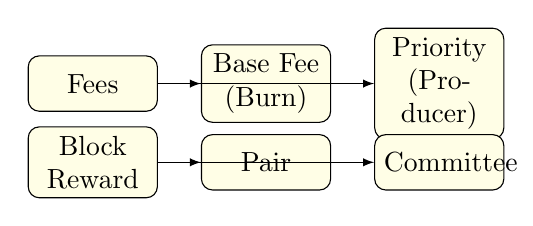
\begin{tikzpicture}[node distance=1cm, auto,
    box/.style={rectangle, draw, fill=yellow!10, text width=4em, text centered, rounded corners, minimum height=2em},
    line/.style={draw, -latex}]
\node [box] (fees) {Fees};
\node [box, right of=fees, xshift=1.2cm] (base) {Base Fee (Burn)};
\node [box, right of=base, xshift=1.2cm] (prio) {Priority (Producer)};
\node [box, below of=fees] (reward) {Block Reward};
\node [box, right of=reward, xshift=1.2cm] (pair) {Pair};
\node [box, right of=pair, xshift=1.2cm] (comm) {Committee};
\path [line] (fees) -- (base);
\path [line] (fees) -- (prio);
\path [line] (reward) -- (pair);
\path [line] (reward) -- (comm);
\end{tikzpicture}
\caption{PAI fee and reward distribution}
\label{fig:economics}
\end{figure}

\section{Validation, Attestation \& Cross-Verification}
\subsection{Block-Relevant State Construction}
For each block, nodes construct a view containing only touched elements:
\begin{itemize}
\item Touched accounts
\item Touched assets
\item Touched debt instruments
\end{itemize}

Cryptographic commitments over these sets enable efficient verification without scanning full history.

\subsection{Attestation Process}
The paired validator validates all transactions against the block-relevant view and produces an attestation containing block identifier, validator identity, validity status, and cryptographic signature.

\subsection{Cross-Verification}
The block producer receives the attestation and verifies it against its own view of the shared replicated ledger. Both parties reference identical ledger state, simplifying cross-verification. Disagreements trigger slashing mechanisms.

\section{Reputation \& Slashing}
\subsection{Reputation System}
Reputation determines committee selection weight and reflects participant reliability. Factors include:
\begin{itemize}
\item \textbf{Uptime}: Node availability and responsiveness
\item \textbf{Success rate}: Successful attestations and valid participation
\item \textbf{Recency decay}: Recent behavior weighted more heavily with time-based decay
\item \textbf{Stake consideration}: Bonded stake influences reputation weighting
\end{itemize}

Reputation decays over time according to:
\begin{equation}
R_{t+1} = R_t \cdot \delta + \Delta_t, \quad \delta \approx 0.99
\end{equation}

where $\Delta_t$ represents reputation changes from observed behavior.

\subsection{Slashing}
Slashing penalties are scaled by severity:

\begin{table}[H]
\centering
\begin{tabular}{lcc}
\toprule
\textbf{Severity} & \textbf{Penalty} & \textbf{Consequence} \\
\midrule
Minor & Partial bond slash & Temporary penalty \\
Major & Substantial bond slash & Significant penalty \\
Critical & Full bond slash & Permanent removal from bonded set \\
\bottomrule
\end{tabular}
\caption{Slashing severity levels}
\label{tab:slashing}
\end{table}

Slashable offenses include:
\begin{enumerate}
\item Block producer accepting or verifying false validator claims against the shared replicated ledger
\item Validator producing false attestations
\end{enumerate}

\subsection{Committee Selection}
Committee members are selected via reputation-weighted selection from non-paired eligible participants, favoring high-reputation, reliable nodes while maintaining decentralization.

\section{Security Considerations}
\subsection{Economic Security}
\begin{itemize}
\item Bonding requirements ensure economic stake in honest behavior
\item Slashing creates cost for malicious actions
\item Auction mechanism prevents predictable block production
\item Committee provides additional oversight against pair collusion
\end{itemize}

\subsection{Debt Enforcement}
\begin{itemize}
\item Immutable history prevents debt record tampering
\item One-transaction settlement prevents partial debt evasion
\item Automatic burning enforces consequences for failed settlements
\item Liquidation escalation provides multiple recovery paths
\end{itemize}

\subsection{Consensus Security}
\begin{itemize}
\item Shared replicated ledger enables cross-verification
\item Pairwise attestation with committee quorum prevents unilateral actions
\item Sealed-bid auction prevents front-running of selection
\item Reputation system incentivizes long-term honest participation
\end{itemize}

\subsection{Invariant Enforcement}
Critical invariants maintained by the protocol:
\begin{itemize}
\item Debt history remains immutable
\item Burned instruments and currencies are permanently destroyed
\item Full debt payment required for instrument transfer or burn triggered
\item Slashing conditions are enforced objectively
\item Block-relevant validation maintains consistency with shared ledger
\end{itemize}

\section{Conclusion}
PAI introduces a fundamentally different approach to blockchain design by embedding debt as a native primitive. The combination of debt instruments, strict transfer mechanics, liquidation mechanisms, and custom consensus creates a system purpose-built for debt-based economic activity. The shared replicated ledger architecture with block-relevant validation balances security and efficiency, while the economic model aligns incentives through bonding, reputation, slashing, and dynamic fee mechanisms. The protocol provides a complete framework for debt creation, enforcement, and resolution without relying on layered smart contract systems for core debt logic.

\section{References}
\begin{enumerate}
\item Nakamoto, S. (2008). Bitcoin: A Peer-to-Peer Electronic Cash System.
\item Buterin, V. et al. (2015). Ethereum: A Next-Generation Smart Contract and Decentralized Application Platform.
\item Buterin, V. (2019). Ethereum Improvement Proposal 1559: Fee Market Change for ETH 1.0 Chain.
\item Wood, G. (2014). Ethereum: A Secure Decentralised Generalised Transaction Ledger.
\end{enumerate}

\section{Appendix}
\subsection{Key Parameters}
\begin{table}[H]
\centering
\begin{tabular}{lc}
\toprule
\textbf{Parameter} & \textbf{Value} \\
\midrule
Committee Size & 4 \\
Minor Slash & 10\% of bond \\
Major Slash & 50\% of bond \\
Critical Slash & 100\% of bond \\
Default Interest Rate & 5\% (500 bps) \\
Liquidation Threshold & 80\% (8000 bps) \\
Reputation Decay Factor & 0.99 \\
Target Gas Usage & Protocol defined \\
\bottomrule
\end{tabular}
\caption{Core protocol parameters}
\label{tab:params}
\end{table}

\subsection{Glossary}
\begin{description}
\item[Debt Instrument] A protocol-level record tracking collateral, debt obligations, and history for a deposit.
\item[Block-Relevant Validation] Validation limited to state elements touched by transactions in the current block.
\item[Custom Attested Bundle] Consensus mechanism combining sealed-bid auctions, pairwise production, and committee attestation.
\item[Shared Replicated Ledger] Canonical ledger state maintained identically across all network participants.
\item[Value Factor] Ratio-based metric representing instrument value relative to minted currencies and collateral.
\item[Liquidation Pool] Aggregate liquidity pool with provider instrument and fungible shares for debt resolution.
\item[Bounty] Auctioned value created when a depositor withdraws while loans remain unpaid.
\item[Consistency Score] Fraction of affected loans repaid at withdrawal, used to shorten bounty time limits.
\end{description}

\end{document}
